\section{MPC regulátor}
Ako už bolo v úvode spomenuté, práca spája viacero odborov do jednej implementácie. Táto časť preto je venovaná návrhu a overenia MPC regulátora.
\subsection{Teoretický základ MPC}
V tejto časti sa vysvetlí história, matematický základ a variácie MPC regulátora.
\subsubsection{On-line MPC}
Prediktívny regulátor je, na najnižšej úrovni, metóda riadenia dynamických systémov, ktorá využíva nástroje matematickej optimalizácie. Spoločné črty všetkých prístupov riešenia problému prediktívnych regulátorov je vypočítať on-line, v každej časovej vzorke,  optimálny riadiaci zásah v konečnom horizonte predikcie pre dynamický model systému, kde aktuálny stav je počiatočný stav. Iba prvý element z vypočítanej sekvencie predikovaných riadiacich zásahov je potom aplikovaný na systém. V ďalšom okamihu vzorkovania je horizont predikcie posunutý a výpočet optimálneho riadiaceho zásahu je vykonávaný znovu pre novonadobudnutý stav. Táto myšlienka nie je nová, už v článku od Lee a Markus (1967), je možné nájsť nasledujúce tvrdenie: ,,Jedna technika na návrh regulátora so spätnou väzbou zo znalosti regulátora pre otvorenú slučku je merať aktuálny stav riadenia procesu a veľmi rýchlo vypočítať funkciu riadenia pre otvorenú slučku. Prvá časť tejto funkcie je potom využitá počas krátkeho intervalu, po ktorom je opäť zmeraný stav procesu a k nemu vypočítaná riadiaca funkcia pre otvorenú slučku. Táto procedúra je potom opakovaná.`` Technika popisovaná v článku od Lee a Markus (1967) je zvyčajne označovaná ako ,,Receding Horizon Control`` (RHC) – ,,Postupujúci horizont riadenia`` a dnes je viac-menej používaný ako synonymum k pojmu,,Model Predictive Control`` – ,,Prediktívne riadenie``. \cite{MPC03} Popisovaný princíp je znázornený na obrázku \ref{01_rec_horizon}.
\begin{figure}[h]
\centering
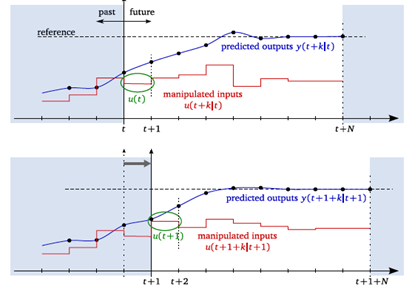
\includegraphics[width=0.75\textwidth]{01_rec_horizon.png}
\caption{Postupujúci horizont riadenia}
\label{01_rec_horizon}
\end{figure}
Nech existuje lineárny dynamický model s časovo invariantnými parametrami, vyjadrený diskrétnou stavovou rovnicou:
\begin{equation} \label{eq1}
\begin{split}
x(t+1)=Ax(t)+Bu(t), \\
y(t)=Cx(t)+Du(t), \\
x(t)∈R^n, y(t)∈R^P, u(t)∈R^m, \\
A∈R^{(n×n)}, B∈R^{(n×m)}, C∈R^{(p×n)}
\end{split}
\end{equation}
x, y, u sú stavy systému, výstupy systému a riadiace zásahy v uvedenom poradí v čase alebo lepšie povedané vo vzorke t. \\
n – predstavuje počet stavov systému \\
p – predstavuje počet výstupov \\
m – predstavuje počet vstupov \\
Matice A, B, C sú systémová matica, vstupná matica a výstupná matica v uvedenom poradí. System \ref{eq1} musí spĺňať nasledujúce obmedzenia na stav a vstup:
\begin{equation} \label{eq2}
\begin{split}
x(t)∈X,u(t)∈U \\
U⊂R^m \\
X⊂R^n
\end{split}
\end{equation}
kde obmedzujúca množina riadiacich zásahov U je konvexná, kompaktná (uzavretá a ohraničená) a obmedzujúca množina stavov X je konvexná a uzavretá. Pre obidve množiny U a X sa predpokladá, že obsahujú počiatok v ich vnútri.\cite{MPC04}
Najskôr je jednoduchšie vyriešiť optimálne riadenie bez obmedzení. Pozornosť bude upriamená na nájdenie takej optimálnej postupností $u^*$(k), ..., $u^*$(k+N – 1), ktorá bude minimalizovať zvolené kvadratické kritérium a zároveň rešpektovať dynamiku systému. Čo inými slovami znamená, že tento regulátor sa bude snažiť minimalizovať stav a rovnako riadiaci zásah, ešte lepšie povedané ich kvadrát. Ak by teda nebola špecifikovaná referenčná hodnota, ktorú má výstup regulátora sledovať, tak implicitne výstupná veličina prediktívneho regulátora konverguje k hodnote 0 alebo pri systémoch s viacerými výstupmi k nulovému vektoru.\\
N – predstavuje horizont predikcie. Ak je teda systém v stave $x_0$, ktorý poznáme a horizont predikcie je 3, tak do optimalizačnej funkcie vstupujú premenné $x_1$, $x_2$, $x_3$ a $u_1$, $u_2$, $u_3$ kde $u_1$ zabezpečí prechod do stavu $x_1$, $u_2$ do stavu $x_2$ atď. každá premenná x je odvoditeľná z predošlého stavu a prvý stav $x_0$ je známy. Preto jedinou ,,neznámou`` ostáva sekvencia riadiacich zásahov. Jedna z otázok by mohla byť, prečo sa využíva kvadratické kritérium. Ako odpoveď je možné použiť príklad kvality riadenia. Pri hodnotení kvality riadenia sa používajú integrálne kritéria. Existuje jednoduché kritérium, ktoré spraví integrál pod krivkou regulačnej odchýlky. Nevýhodou tohto je, že ak dochádza k preregulovaniu a regulačná odchýlka je záporná, veľkosť plochy je zmenšovaná o tie časti, ktoré sú záporné. Toto sa rieši absolútnym integrálnym kritériom, ktoré spraví zo zápornej regulačnej odchýlky kladnú a teda plocha pod krivkou sa zväčšuje aj pri preregulovaní. Navyše existuje kvadratické kritérium, ktoré okrem toho, že odstraňuje problém so zápornou regulačnou odchýlkou navyše viac penalizuje hodnoty odchýlky väčšie ako 1. Inými slovami, ak je hodnota viac ako 1 o to horšiu kvalitu regulácie bude toto kritérium indikovať. Problém so zápornou regulačnou odchýlkou je znázornený na obrázkoch \ref{02_reg_odch}, \ref{03_reg_odch} a \ref{04_reg_odch}.
\begin{figure}[h]
\centering
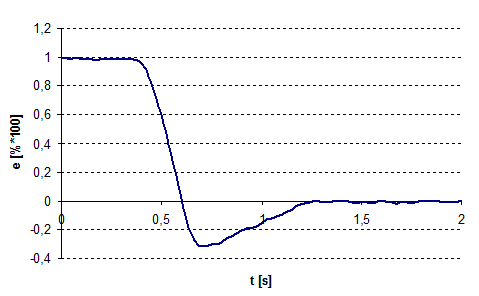
\includegraphics[width=0.90\textwidth]{02_reg_odch.png}
\caption{Hodnota regulačnej odchýlky v čase}
\label{02_reg_odch}
\end{figure}

\begin{figure}[h]
\centering
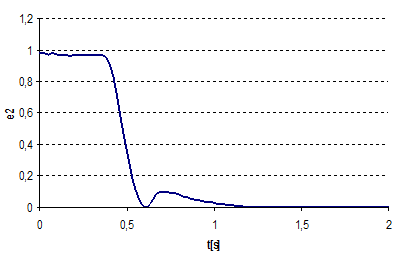
\includegraphics[width=0.90\textwidth]{03_reg_odch.png}
\caption{Časová závislosť kvadrátu regulačnej odchýlky}
\label{03_reg_odch}
\end{figure}
\begin{figure}[h]
\centering
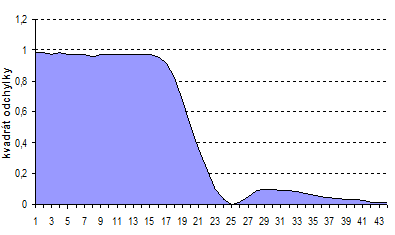
\includegraphics[width=0.90\textwidth]{04_reg_odch.png}
\caption{Plocha kvadrátu regulačnej odchýlky}
\label{04_reg_odch}
\end{figure}

Rovnako ako pri minimalizácii regulačnej odchýlky, tak aj pri minimalizácii riadiaceho zásahu je kvadratické kritérium najlepším ukazovateľom. \\
Pre porozumenie ďalších vzťahov si je potrebné uvedomiť, že: $x(t+k) =x_{(t+k)}$ \\
\begin{itemize}
\item Pre vzorku k = 0 (aktuálny stav systému): x(t)= $x_t$, 
\item pre vzorku k = 1 x(t+1)=$x_{(t+1)}$, 
\item atď.
\end{itemize}
Kvadratické kritérium pre konečný horizont predikcie dĺžky N je:
\begin{equation} \label{eq3}
\begin{split}
J(x(t),u(t),…,u(N-1))=\frac{1}{2}∑_{k=0}^{N-1}[x_k^T Qx_k+u_k^T Ru_k ] +  \frac{1}{2} x_N^T Q_N x_N
\end{split}
\end{equation}
kde:
\begin{equation} \label{eq4}
\begin{split}
x_(k+1)=Ax_k+Bu_k \\
x_0=x(t), \\
Q=Q^T  \succcurlyeq 0,Q_N=Q_N^T \succcurlyeq 0,R=R^T \succ 0 \\
Q_N∈R^{n×n} \\
R∈R^{m×m}
\end{split}
\end{equation}
Matice, Q, $Q_N$ a R sú nazývané váhové matice a spolu s horizontom predikcie N sú nazývané parametrami na ladenie prediktívneho regulátora. Nájdenie optimálneho riadenia, ktoré by minimalizovalo kvadratické kritérium predstavuje dynamickú optimalizáciu a má v tomto prípade aj analytické riešenie: \cite{MPC05}

\begin{equation} \label{eq5}
\begin{split}
x_{t+k}= A^k x_0+ ∑_{i=0}^{k-1}A^i Bu_{k-1-i}\\
u_{t,N}=[u_t^T,…,u_{t+N-1}^T  ]
\end{split}
\end{equation}

Vyjadrenie predikovaného stavu je potom:
\begin{equation} \label{eq6}
\begin{split}
[ x_{t+1}^T,…,x_{t+N}^T  ]^T=Vx_0+Tu_{t,N}
\end{split}
\end{equation}

Táto rovnica je jedna z najdôležitejších pri pochopení fungovania on-line prediktívneho algoritmu. Preto je vhodné ukázať ako matica V a T vyzerajú pre konkrétny jednoduchý systém s horizontom predikcie N = 3 zadaný v stavovom priestore:

\begin{equation} \label{eq7}
\begin{split}
A = \begin{bmatrix}
1 & 0 \\
1 & 1 \\
\end{bmatrix}, 
B = \begin{bmatrix}
0 \\
0,5 \\
\end{bmatrix} \\
C = \begin{bmatrix}
0 & 1 \\
\end{bmatrix}, D = 0 \\
x_{0} = \begin{bmatrix}
4 \\
5 \\
\end{bmatrix} = \begin{bmatrix}
x_{01} \\
x_{02} \\
\end{bmatrix}
\end{split}
\end{equation}
Matice V~a~T budú vyzerať:
\begin{equation} \label{eq8}
\begin{split}
V = \begin{bmatrix}
\begin{matrix}
1 & 0 \\
1 & 1 \\
\end{matrix} \\
\begin{matrix}
1 & 0 \\
2 & 1 \\
\end{matrix} \\
\begin{matrix}
1 & 0 \\
3 & 1 \\
\end{matrix} \\
\end{bmatrix} = \begin{bmatrix}
A^{1} \\
A^{2} \\
A^{3} \\
\end{bmatrix} \\
T = \begin{bmatrix}
\begin{matrix}
1 & 0 & 0 \\
0,5 & 0 & 0 \\
\end{matrix} \\
\begin{matrix}
1 & 1 & 0 \\
1,5 & 0,5 & 0 \\
\end{matrix} \\
\begin{matrix}
1 & 1 & 1 \\
2,5 & 1,5 & 0,5 \\
\end{matrix} \\
\end{bmatrix} = \begin{bmatrix}
\begin{matrix}
A^{0}B & 0\  & 0 \\
\end{matrix} \\
\begin{matrix}
A^{1}B & A^{0}B & 0 \\
\end{matrix} \\
\begin{matrix}
A^{2}B & A^{1}B & A^{0}B \\
\end{matrix} \\
\end{bmatrix}
\end{split}
\end{equation}

Výsledný vzťah:
\begin{equation} \label{eq9}
\begin{split}
{\lbrack\ \begin{bmatrix}
x_{11} \\
x_{12} \\
\end{bmatrix},\ \begin{bmatrix}
x_{21} \\
x_{22} \\
\end{bmatrix},\begin{bmatrix}
x_{31} \\
x_{32} \\
\end{bmatrix}\rbrack}^{T} = \begin{bmatrix}
A^{1} \\
A^{2} \\
A^{3} \\
\end{bmatrix}\begin{bmatrix}
x_{01} \\
x_{02} \\
\end{bmatrix} + \begin{bmatrix}
\begin{matrix}
A^{0}B & 0\  & 0 \\
\end{matrix} \\
\begin{matrix}
A^{1}B & A^{0}B & 0 \\
\end{matrix} \\
\begin{matrix}
A^{2}B & A^{1}B & A^{0}B \\
\end{matrix} \\
\end{bmatrix}\begin{bmatrix}
u_{1} \\
u_{2} \\
u_{3} \\
\end{bmatrix}
\end{split}
\end{equation}
Dôležitý krok pri hľadaní optimálneho riadenia je zo vzťahu \ref{eq3}
„odstrániť`` sumu. Finálny vzťah vyzerá:
\begin{equation} \label{eq10}
\begin{split}
J\left( x\left( t \right),U_{t} \right) = \ \frac{1}{2}{u_{t,N}}^{T}Hu_{t,N} + x^{T}\left( t \right)FU_{t} + \frac{1}{2}x^{T}\left( t \right)\text{Yx}\left( t \right),
\end{split}
\end{equation}

Matica \(\ H \in R^{(m \bullet N \times m \bullet N)}\) ,
\(F \in R^{(n \times m \bullet N)}\), \(Y \in R^{(n \times n)}\). Ak sa
symbol \(\bigotimes\) označí ako kroneckerovo násobenie matíc a
\(I_{j} \in R^{(j \times j)}\), jednotková matica s~príslušnou
dimenziou, tak platí:

\begin{equation} \label{eq11}
\begin{split}
H = \ T^{T}\tilde{Q}T + \ I_{N}\ \bigotimes\ R,\ \ F = V^{T}\tilde{Q}T,\ \ Y = V^{T}\tilde{Q}V \\
\tilde{Q} = \ \begin{bmatrix}
I_{N - 1}\ \bigotimes\ Q & 0 \\
0 & Q_{N} \\
\end{bmatrix}
\end{split}
\end{equation}

Pre systém zo vzťahu \ref{eq7} a~váhy \(Q = Q_{N} = I_{2},\ R = 0,1\) budú
jednotlivé matice vyzerať:

\begin{equation} \label{eq12}
\begin{split}
H = \ \begin{bmatrix}
11,85 & 6,5 & 2,25 \\
6,5 & 4,6 & 1,75 \\
2,25 & 1,75 & 1,35 \\
\end{bmatrix}, F = \begin{bmatrix}
14 & 7,5 & 2,5 \\
4,5 & 2 & 0,5 \\
\end{bmatrix}, \\
Y = \ \ \begin{bmatrix}
17 & 6 \\
6 & 3 \\
\end{bmatrix}
\end{split}
\end{equation}

Optimálnu riadiacu sekvenciu je možné dostať minimalizáciou kvadratickej
formy \ref{eq10}:

\begin{equation} \label{eq13}
\begin{split}
u_{t,N}^{*}\left( x\left( t \right) \right) = \arg{\min_{u_t,N}{\{ J(x\left( t \right),u_{t,N}\ \}}} = - H^{- 1}F^{T}x(t)
\end{split}
\end{equation}

Optimálna hodnota kritéria je:

\begin{equation} \label{eq14}
\begin{split}
J^{*}\left( x\left( t \right) \right) = \min_{u_t,N}{\{ J(x\left( t \right),u_{t,N}\ \}} = \frac{1}{2}x^{T}(t)(Y - FH^{- 1}F^{T})x(t)
\end{split}
\end{equation}

Na to aby sa zabezpečila spätná väzba, je potrebné v~každom kroku použiť
iba prvú hodnotu zo sekvencie riadiacich zásahov a~potom zmerať stav
a~na základe tej hodnoty znovu vypočítať optimálnu sekvenciu riadiacich
zásahov. Bez merania stavu, by to bola regulácia v~otvorenom regulačnom
obvode. Meranie stavu a~jeho použitie pri výpočte nasledujúceho
riadiaceho zásahu v~každom kroku zabezpečí reguláciu v~uzavretom
regulačnom obvode.

\subsubsection{On-line MPC s obmedzením}

Doteraz sa reguloval systém, v~ktorom nebolo žiadne obmedzenie.
V~realite ich však býva mnoho. Pokiaľ sa pri návrhu regulátora začnú
brať do úvahy rovnice \ref{eq2}, bude ich treba zapracovať do výpočtu. Pri
návrhu prediktívneho regulátora s~obmedzením sa využíva kvadratické
programovanie. Úloha kvadratického programovania je úlohou nelineárneho
programovania, v~ktorej sústava ohraničení je lineárna a~účelová funkcia
je kvadratická. Všeobecná formulácia kvadratickej úlohy je:

\begin{equation} \label{eq15}
\begin{split}
f\left( x \right) = \min_{x}\left\{ x^{T}Hx + F^{T}\text{x\ } \right\} \\
x \in D = \{\operatorname{x|}{\ \ Lx \leq m_{c}},\ x \geq 0\}
\end{split}
\end{equation}

Pre návrh regulátora je premenná, ktorej minimum sa hľadá, sekvencia
riadiacich zásahov \(u_{t,N}^{*}\). Rovnice pre prediktívny regulátor
s~obmedzením následne vyzerajú:

\begin{equation} \label{eq16}
\begin{split}
J\left( x\left( t \right),\ u\left( t \right),\ldots,\ u\left( N - 1 \right) \right) = \frac{1}{2}\sum_{k = 0}^{N - 1}\left\lbrack x_{k}^{T}Qx_{k} + u_{k}^{T}Ru_{k} \right\rbrack + \ \frac{1}{2}x_{N}^{T}Q_{N}x_{N}
\end{split}
\end{equation}

kde:
\begin{equation} \label{eq17}
\begin{split}
x_{k + 1} = Ax_{k} + Bu_{k}, \\
x_{0} = x\left( t \right), \\
E_{c}x_{k} + G_{c}u_{k} \leq m_{c},\ \ k = 1\ldots N \\
Q = Q^{T} \succcurlyeq 0,\ Q_{N} = Q_{N}^{T} \succcurlyeq 0,\ R = R^{T} \succ 0
\end{split}
\end{equation}

Aby bolo možné sústavu rovníc \ref{eq16} a \ref{eq17} zapracovať do kvadratického programovania, previesť do maticového tvaru. Prvá časť rovnice ostáva nezmenená, pridá sa k~nej druhá časť:

\begin{equation} \label{eq18}
\begin{split}
J\left( x\left( t \right),U_{t} \right) = \ \frac{1}{2}{u_{t,N}}^{T}Hu_{t,N} + x^{T}\left( t \right)FU_{t} + \frac{1}{2}x^{T}\left( t \right)\text{Yx}\left( t \right), \\
Gu_{t,N} \leq w + Ex(t)
\end{split}
\end{equation}

Kde matice H, F, Y sú určené rovnako ako vo vzťahu \ref{eq11} a~matice G, E, a
vektor w majú tvar:

\begin{equation} \label{eq19}
\begin{split}
G = \begin{bmatrix}
{- I}_{N} \\
\begin{matrix}
I_{N} \\
 - (I_{N}\bigotimes CT) \\
\end{matrix} \\
\begin{matrix}
(I_{N}\bigotimes CT) \\
 \vdots \\
\end{matrix} \\
\end{bmatrix},\ E = \begin{bmatrix}
0 \\
\begin{matrix}
0 \\
 - (I_{N}\bigotimes CV) \\
\end{matrix} \\
\begin{matrix}
(I_{N}\bigotimes CV) \\
 \vdots \\
\end{matrix} \\
\end{bmatrix},\ w = \begin{bmatrix}
 - (1_{N}\bigotimes u_{\min}) \\
\begin{matrix}
(1_{N}\bigotimes u_{\max}) \\
 - (1_{N}\bigotimes y_{\min}) \\
\end{matrix} \\
\begin{matrix}
(1_{N}\bigotimes y_{\max}) \\
 \vdots \\
\end{matrix} \\
\end{bmatrix}
\end{split}
\end{equation}

V rovnici \ref{eq19} sú znázornené základné systémové obmedzenia. Môže
existovať ďaleko viac. \(1_{N}\) predstavuje jednotkový vektor
o~veľkosti N. Prvé dva riadky matice G, \(G_{1,2} \in R^{N \times N}\),
E, \(E_{1,2} \in R^{N \times n}\) a~vektor W, \(W_{1,2} \in R^{N}\) v
(19) predstavujú obmedzenia vstupu. Druhé dva riadky matice G,
\(G_{3,4} \in R^{N \times N}\), E, \(E_{3,4} \in R^{N \times n}\)
a~vektor W, \(W_{3,4} \in R^{N}\) v \ref{eq19} predstavujú obmedzenia výstupu.
Ďalšie obmedzenia, by museli nadobúdať rovnaké rozmery ako predošlé
riadky príslušných matíc a~vektora.

Ak sa pridajú do systému \ref{eq7} obmedzenia na vstup a~výstup:

\begin{equation} \label{eq20}
\begin{split}
- 1 \leq u\left( t \right) \leq 1,\ \  - 10 \leq y\left( t \right) \leq \ 10
\end{split}
\end{equation}

matice G, E a vektor~w budú vyzerajú:

\begin{equation} \label{eq21}
\begin{split}
G = \begin{bmatrix}
{- I}_{3} \\
I_{3} \\
\begin{matrix}
 - (I_{3}\bigotimes CT) \\
(I_{3}\bigotimes CT) \\
\end{matrix} \\
\end{bmatrix},\ E = \begin{bmatrix}
0 \\
\begin{matrix}
0 \\
 - (I_{3}\bigotimes CV) \\
\end{matrix} \\
\begin{matrix}
(I_{3}\bigotimes CV) \\
 \vdots \\
\end{matrix} \\
\end{bmatrix},\ m_{c} = \begin{bmatrix}
 - (1_{3}\bigotimes u_{\min}) \\
(1_{3}\bigotimes u_{\max}) \\
\begin{matrix}
 - (1_{3}\bigotimes y_{\min}) \\
(1_{3}\bigotimes y_{\max}) \\
\end{matrix} \\
\end{bmatrix}
\end{split}
\end{equation}

\begin{equation} \label{eq22}
\begin{split}
G = \begin{bmatrix}
 - \begin{pmatrix}
1 & 0 & 0 \\
0 & 1 & 0 \\
0 & 0 & 1 \\
\end{pmatrix} \\
\begin{pmatrix}
1 & 0 & 0 \\
0 & 1 & 0 \\
0 & 0 & 1 \\
\end{pmatrix} \\
\begin{matrix}
 - \begin{pmatrix}
0,5 & 0 & 0 \\
1,5 & 0,5 & 0 \\
2,5 & 1,5 & 0,5 \\
\end{pmatrix} \\
\begin{pmatrix}
0,5 & 0 & 0 \\
1,5 & 0,5 & 0 \\
2,5 & 1,5 & 0,5 \\
\end{pmatrix} \\
\end{matrix} \\
\end{bmatrix},\ E = \begin{bmatrix}
 - \begin{pmatrix}
0 & 0 \\
0 & 0 \\
0 & 0 \\
\end{pmatrix} \\
\begin{pmatrix}
0 & 0 \\
0 & 0 \\
0 & 0 \\
\end{pmatrix} \\
\begin{matrix}
 - \begin{pmatrix}
1 & 1 \\
2 & 1 \\
3 & 1 \\
\end{pmatrix} \\
\begin{pmatrix}
1 & 1 \\
2 & 1 \\
3 & 1 \\
\end{pmatrix} \\
\end{matrix} \\
\end{bmatrix},\ w = \begin{bmatrix}
\begin{pmatrix}
1 \\
1 \\
\end{pmatrix} \\
\begin{pmatrix}
1 \\
1 \\
\end{pmatrix} \\
\begin{matrix}
\begin{pmatrix}
10 \\
10 \\
\end{pmatrix} \\
\begin{pmatrix}
10 \\
10 \\
\end{pmatrix} \\
\end{matrix} \\
\end{bmatrix}
\end{split}
\end{equation}

Vznikne sústava lineárnych rovníc, ktoré tvoria obmedzenia pre
kvadratický problém.

\begin{equation} \label{eq23}
\begin{split}
\begin{bmatrix}
 - \begin{pmatrix}
1 & 0 & 0 \\
0 & 1 & 0 \\
0 & 0 & 1 \\
\end{pmatrix} \\
\begin{pmatrix}
1 & 0 & 0 \\
0 & 1 & 0 \\
0 & 0 & 1 \\
\end{pmatrix} \\
\begin{matrix}
 - \begin{pmatrix}
0,5 & 0 & 0 \\
1,5 & 0,5 & 0 \\
2,5 & 1,5 & 0,5 \\
\end{pmatrix} \\
\begin{pmatrix}
0,5 & 0 & 0 \\
1,5 & 0,5 & 0 \\
2,5 & 1,5 & 0,5 \\
\end{pmatrix} \\
\end{matrix} \\
\end{bmatrix}\begin{bmatrix}
u_{1} \\
u_{2} \\
u_{3} \\
\end{bmatrix} \leq \begin{bmatrix}
\begin{pmatrix}
1 \\
1 \\
\end{pmatrix} \\
\begin{pmatrix}
1 \\
1 \\
\end{pmatrix} \\
\begin{matrix}
\begin{pmatrix}
10 \\
10 \\
\end{pmatrix} \\
\begin{pmatrix}
10 \\
10 \\
\end{pmatrix} \\
\end{matrix} \\
\end{bmatrix} + \begin{bmatrix}
 - \begin{pmatrix}
0 & 0 & 0 \\
0 & 0 & 0 \\
0 & 0 & 0 \\
\end{pmatrix} \\
\begin{pmatrix}
0 & 0 & 0 \\
0 & 0 & 0 \\
0 & 0 & 0 \\
\end{pmatrix} \\
\begin{matrix}
 - \begin{pmatrix}
1 & 1 \\
2 & 1 \\
3 & 1 \\
\end{pmatrix} \\
\begin{pmatrix}
1 & 1 \\
2 & 1 \\
3 & 1 \\
\end{pmatrix} \\
\end{matrix} \\
\end{bmatrix}\begin{bmatrix}
x_{01} \\
x_{02} \\
\end{bmatrix}
\end{split}
\end{equation}

Ak sú obmedzenia na systém príliš striktné, môže sa stať, že kvadratický
problém nemá riešenie. Takáto situácia je znázornená na obrázku \ref{05_restric}.

\begin{figure}[h]
\centering
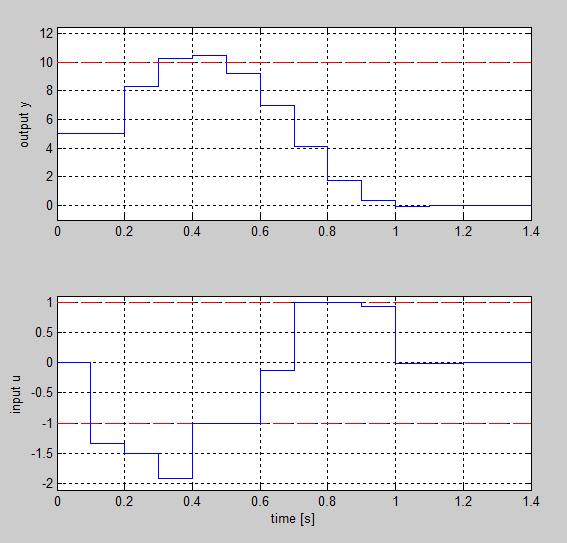
\includegraphics[width=0.99\textwidth]{05_restric.png}
\caption{Časový priebeh výstupnej veličiny a riadiaceho zásahu pre neriešiteľný kvadratický problém. Červená čiara predstavuje obmedzenie na danú veličinu}
\label{05_restric}
\end{figure}

Ak by obmedzenia na výstup boli napríklad
\(- 13 \leq y\left( t \right) \leq \ 13\), kvadratický problém by bol
riešiteľný a~jeho riešenie pre horizont predikcie 3 je zobrazene na
obrázku \ref{06_restric_ok}.

\begin{figure}[h]
\centering
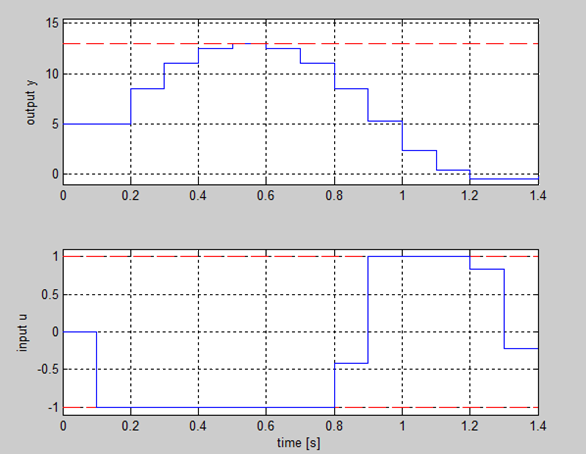
\includegraphics[width=0.99\textwidth]{06_restric_ok.png}
\caption{Časový priebeh výstupnej veličiny a riadiaceho zásahu riešiteľného kvadratického problému}
\label{06_restric_ok}
\end{figure}

\subsubsection{On-line MPC so sledovaním referenčného signálu}
Doteraz bol riešený regulátor, ktorý reguloval hodnotu k „počiatku``
k~hodnote 0 alebo nulovému vektoru. Táto kapitola obsahuje návrh MPC
regulátora, ktorý bude sledovať po častiach konštantný referenčný signál
r(t). Stále sa berie do úvahy systém \ref{eq1}. Najprv je potrebné nahradiť
člen \(x_{k}^{T}Qx_{k}\) v~pôvodnom kritériu \ref{eq17} odchýlkou

\begin{equation} \label{eq24}
\begin{split}
{(z_{k} - r_{k})}^{T}Q_{y}(z_{k} - r_{k})
\end{split}
\end{equation}

kde

\begin{equation} \label{eq25}
\begin{split}
z\left( t \right) = Zy\left( t \right),\ z\left( t \right) \in R^{p_{z}},\ p_{z} \leq p,\ r \leq m
\end{split}
\end{equation}

Aby to bolo možné, je potrebné poznať predikovanú hodnotu referenčného
signálu. Ta môže byť definovaná rôznymi spôsobmi jedna z~možností:
r(t+1)=r(t).

V~ustálenom stave je potrebné, aby platila rovnosť \(z_{u} = r_{u}\).
Takže:

\begin{equation} \label{eq26}
\begin{split}
\begin{bmatrix}
I_{n} - A & - B \\
\text{ZC} & 0 \\
\end{bmatrix}\ \begin{bmatrix}
x_{u} \\
u_{u} \\
\end{bmatrix} = \begin{bmatrix}
0 \\
r_{u} \\
\end{bmatrix}
\end{split}
\end{equation}


Ak ma predchádzajúca matica plnú riadkovú hodnosť, existuje riešenie \(u_{u}\)
a \(x_{u}.\). V~dôsledku nenulového ustáleného vstupu sa v~praxi často
používa odchýlka \(u_{k} = u_{k} - u_{k - 1}\). Ak sústava obsahuje
integrátor, je lepšie použiť hodnotu u. \cite{MPC05}

Kritérium pre sledovanie referencie má tvar:

\begin{equation} \label{eq27}
\begin{split}
J\left( x\left( t \right),\ u\left( t \right),\ldots,\ u\left( N - 1 \right) \right) = \frac{1}{2}\sum_{k = 0}^{N - 1}\left\lbrack e_{k}^{T}Q_{e}e_{k} + u_{k}^{T}Ru_{k} \right\rbrack
\end{split}
\end{equation}

kde 

\begin{equation} \label{eq28}
\begin{split}
e_{k} = y_{k} - r_{k}
\end{split}
\end{equation}

je regulačná odchýlka a

\begin{equation} \label{eq29}
\begin{split}
\Delta u_{k} = u_{k} - u_{k - 1}
\end{split}
\end{equation}

je optimalizovaná premenná. Systém rozšírený o~históriu riadiaceho
zásahu \(u_{k}\) a~generátor referencie \(r_{k}\) je formulovaný:

\begin{equation} \label{eq30}
\begin{split}
\begin{bmatrix}
x_{k + 1} \\
u_{k} \\
r_{k + 1} \\
\end{bmatrix} = \begin{bmatrix}
A & B & 0 \\
0 & I_{m} & 0 \\
0 & 0 & I_{n_{y}} \\
\end{bmatrix}\ \begin{bmatrix}
x_{k} \\
u_{k - 1} \\
r_{k} \\
\end{bmatrix} + \begin{bmatrix}
B \\
I_{m} \\
0 \\
\end{bmatrix}u_{k} = \ A_{m}\hat{x_{k}} + B_{m}u_{k} \\
e_{k} = \begin{bmatrix}
C & 0 & - I_{n_{y}} \\
\end{bmatrix}\hat{x_{k}} = C_{m}\hat{x_{k}}
\end{split}
\end{equation}

\begin{figure}[h]
\centering
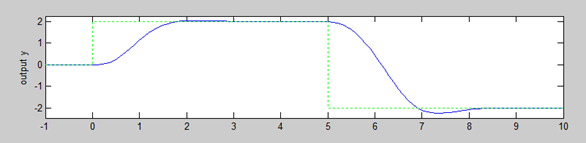
\includegraphics[width=0.99\textwidth]{07_ref.png}
\caption{Sledovanie referencie,  časové priebehy -  zelená referencia, modrá výstup systému}
\label{07_ref}
\end{figure}

Po upravení algoritmu na sledovanie po častiach spojitého referenčného signálu už MPC regulátor neriadi výstupnú veličinu k 0 hodnote alebo vektoru, ale ku aktuálnej hodnote prípadne vektoru referenčného signálu v kroku k, \dots, k + N - 1, kde N predstavuje horizont predikcie. Preto referenčný signál vstupujúci do výpočtu je je buď vektor pre jednorozmerné systémy (SISO) alebo matica pre viacrozmerné systémy (MIMO). Časový priebeh výstupnej veličiny SISO systému regulovaného MPC regulátorom so sledovaním referencie je znázornený na obrázku \ref{07_ref}.

\subsubsection{Explicitné riešenie - offline MPC}

Je zrejmé, že optimálna hodnota kritéria \ref{eq14} a~optimálna riadiaca sekvencia \ref{eq13} (aj s~obmedzeniami) sú funkciou stavu x(t). Túto úlohu je možné formulovať pomocou \textbf{multiparametrického kvadratického
programovania} (mp-QP), ktoré sa snaží nájsť optimálne riešenie pre
všetky možné hodnoty parametra x(t) vopred. Ak sa spraví substitúcia
rovnice

\begin{equation} \label{eq31}
\begin{split}
J^{*}\left( x\left( t \right) \right) = \min_{u_t,N}\left\{ J\left( x\left( t \right),u_{t}) \right|Gu_{t} \leq W + Ex(t) \right\}
\end{split}
\end{equation}

pomocou

\begin{equation} \label{eq32}
\begin{split}
u_{t} = \tilde{u_{t}} - H^{- 1}F^{T}x(t)
\end{split}
\end{equation}

vznikne:

\begin{equation} \label{eq33}
\begin{split}
J^{*}\left( x\left( t \right) \right) = \min_{u_t,N}\left\{ J\left( \tilde{u_{t}},x\left( t \right)) = \frac{1}{2}{\tilde{u}}_{t}^{T}H{\tilde{u}}_{t} + \beta \right|G{\tilde{u}}_{t} \leq W + Sx(t) \right\}
\end{split}
\end{equation}

Kde \(S = E + GH^{- 1}F^{T}\)
a~\(\beta = \frac{1}{2}{x\left( t \right)}^{T}\left( FH^{- 1}F^{T} + Y \right)x(t)\).
Ešte je potrebné zaviesť množinu indexov
I\(= \left\{ 1,\ldots,\ q \right\},\ \)ktorá zodpovedá riadkom matice G,
W a S. \\
Kritický región CR je taká polytopická oblasť v~priestore parametrov
x(t), ktorá má v~optimálnej hodnote
\(J^{*}\left( x\left( t \right) \right),\ u^{*}\left( x\left( t \right) \right)\)
aktívne rovnaké obmedzenia \(A(x(t)) \subset I\). Takže platí

\begin{equation} \label{eq34}
\begin{split}
G_{A}{\tilde{u_{t}}}^{*}\left( x\left( t \right) \right) = W_{A} + S_{A}x\left( t \right)\ pre\ x(t) \in CR
\end{split}
\end{equation}

Nech \(H \succ 0\) a~nech \(G_{A}\)majú lineárne nezávisle riadky, potom
optimálna sekvencia
\({\tilde{u_{t}}}^{*}\left( x\left( t \right) \right)\) je jednoznačne
definovaná afinnou funkciou stavu x(t) na danom kritickom regióne CR.

\begin{equation} \label{eq35}
\begin{split}
{\tilde{u_{t}}}^{*}\left( x\left( t \right) \right) = H^{- 1}G_{A}^{T}(G_{A}H^{- 1}G_{A}^{T})(W_{A} + S_{A}x\left( t \right))
\end{split}
\end{equation}

Ak sa preformuluje optimalizačný problém \ref{eq13} (s obmedzeniami) ako mp-QP
a \(H \succ 0\), potom optimálna riadiaca sekvencia
\({u_{t}}^{*}\left( x\left( t \right) \right):X_{\text{feas}} \rightarrow R^{m}\)
je spojitá, po častiach afinná funkcia na polyedry a~optimálna hodnota
\(J^{*}(x\left( t \right))\) je spojitá, konvexná a~po častiach
kvadratická funkcia na polyedry.

Algoritmus mp-QP najskôr spočíta riešenie (13) (s obmedzeniami) pre
vhodne zvolenú počiatočnú podmienku (\(x_{0} \in X_{\text{feas}}\))
a~vytvorí sa príslušný kritický región CR\textsubscript{0}. Potom
rekurzívne prehľadá okolie a~vytvára nové regióny. Výsledkom je
rozdelenie oblasti \(X_{\text{feas}}\)do kritických regiónov
\(CR_{i} = \left\{ x \right|P_{i}x \leq p_{i}\}\), nad ktorými je
definovaná spojitá afinná funkcia:

\begin{equation} \label{eq36}
\begin{split}
{u_{t}}^{*}\left( x\left( t \right) \right) = F_{i}x\left( t \right) + G_{i}
\end{split}
\end{equation}

a spojitá kvadratická funkcia

\begin{equation} \label{eq37}
\begin{split}
{J_{t}}^{*}\left( x\left( t \right) \right) = x^{T}\left( t \right)A_{i}x\left( t \right) + B_{i}x\left( t \right) + C_{i}
\end{split}
\end{equation}

Týmto sa presunula numerická výpočtová náročnosť optimalizácie \ref{eq13} k~off-line výpočtom. V~priebehu riadenia stačí identifikovať región CR\textsubscript{i}, obsahujúci aktuálny stav x(t) a~aplikovať príslušný
zákon riadenia \label{eq36}. \cite{MPC05} \\
Takýmto spôsobom je možné rozdeliť výpočtovú zložitosť na dve časti. Prvá, výpočtovo zložitejšia, časť je hľadanie kritických regiónov, ktorá sa môže uskutočniť pred zavedením regulátora do behu. Tuto nie je čas kritický, pretože regulačný proces nebeží. Druhá časť je počas behu regulačného procesu. Tá predstavuje časovo nenáročnú operáciu vyhľadania kritického regiónu v pamäti a podľa neho vrátiť akčný zásah. Hlavná nevýhoda offline - explicitného riešenia je, že systém je jednorázovo daný a už počas behu nevstupuje do výpočtu na rozdiel od online riešenia, kde do každého kroku matematický model systému vstupuje a teda je možné  matematický model dynamicky adaptovať, aby čo najviac zodpovedal reálnemu systému. Pri voľbe spôsobu implementácie praktickej časti pre výučbu aj neskôr v IoT prostredí, tento fakt zavážil a zvolila sa online metóda implementácie.

\subsection{Overenie On-line MPC algoritmu}
Po teoretickom základe nasleduje overenie regulátora v programe, ktorý bol vytvorený pre účely využitia v pedagogickom procese v prostredí Matlab a jeho súčasti Guide. Guide slúži na vytváranie grafických rozhraní. Grafické rozhranie vytvoreného programu je znázornené na obrázku \ref{08_gui} 

\begin{figure}[h]
\centering
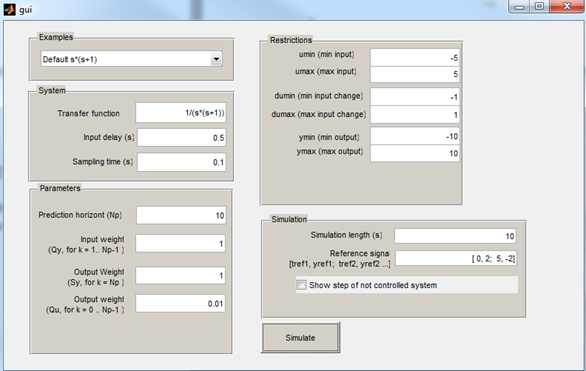
\includegraphics[width=0.99\textwidth]{08_gui.png}
\caption{Grafické rozhranie k programu na testovanie MPC algoritmu.}
\label{08_gui}
\end{figure}

a ponúka pre používateľa možnosti zadania:

\begin{itemize}
\item
  Systémových nastavení:

  \begin{itemize}
  \item
    Automatický vyplniť určité druhy systému
  \item
    Zadať akúkoľvek prechodovú funkciu v~s~alebo z~oblasti systému,
    ktorý má byť riadený
  \item
    Zadať dopravné oneskorenie systému
  \item
    ~periódu vzorkovania
  \end{itemize}
\item
  Ladiace parametre

  \begin{itemize}
  \item
    ~váha vstupu
  \item
    ~váha výstupu pre budúce hodnoty v kroku k=0 \dots N-1, N je horizont predikcie.
  \item
    ~váha výstupu pre budúcu hodnotu v kroku k=N, kde N je horizont predikcie
  \end{itemize}
\item
  Obmedzenia systému

  \begin{itemize}
  \item
    ~minimálny vstup
  \item
    ~maximálny vstup
  \item
    ~minimálna zmena vstupu
  \item
    ~maximálna zmena vstupu
  \item
    minimálny~výstup systému
  \item
    ~maximálny výstup systému
  \end{itemize}
\item
  Parametre simulácie

  \begin{itemize}
  \item
    ~čas simulácie
  \item
    ~referenčný signál zadávaný vo forme vektor dvojice hodnôt, kde prvá
    identifikuje čas, kedy ma zmena nastať a~druhá hodnota veľkosti
    skoku.
  \end{itemize}
\end{itemize}

Výstup z~grafického rozhrania po ponechaní prednastavených hodnôt sú grafy zobrazené na obrázku  \ref{09_out}.

\begin{figure}[h]
\centering
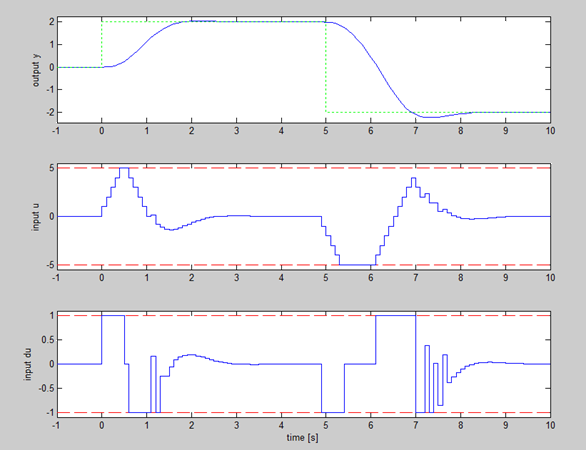
\includegraphics[width=0.99\textwidth]{09_out.png}
\caption{Časové priebehy výstupu systému, riadiaceho zásahu a zmeny riadiaceho zázsahu.}
\label{09_out}
\end{figure}


V~prvom grafe obrázku  \ref{09_out} je znázornený časový priebeh sledovania referenčnej hodnoty výstupnou veličinou. Zelenou farbou je referenčná veličina a výstupna veličina modrou.
V~druhom grafe obrázku  \ref{09_out} je znázornený
riadiaci zásah systému modrou farbou a~obmedzenia riadiaceho zásahu červenou farbou. V~treťom grafe obrázku  \ref{09_out} je znázornená zmena riadiaceho zásahu modrou farbou
a~obmedzenia červenou. Hodnotenie kvality regulácie priamymi ukazovateľmi \cite{MPC06}

\begin{itemize}
  \item Doba regulácie:
    \begin{itemize}
  		\item
    	Pre zmenu v čase 0s (zmena 1.) z hodnoty 0 na 2 je doba regulácie 2 sekundy
    	\item
    	Pre zmenu v čase 5s (zmena 2.) z hodnoty 2 na -2 je doba regulácie 3 sekundy
	\end{itemize}
  \item Preregulovanie:
    \begin{itemize}
  		\item
    	Pre zmenu 1. došlo k minimálnemu preregulovaniu.
    	\item
    	Pre zmenu 2. je preregulovanie badateľné.
	\end{itemize}  
  \item Regulačná odchýlka:
    \begin{itemize}
  		\item
    	Regulačná odchýlka je pre oba prípady 0.
	\end{itemize}   
\end{itemize}

Nie je tu porovnanie voči iným regulátorom, pretože to nie je zámerom tejto kapitoly. Kapitola slúži na demonštráciu funkčnosti predchádzajúcej teórie. Čo je však dôležité si na tomto mieste zdôrazniť je znázornenie ako vplývajú obmedzenia na riadenie systému. 

\begin{itemize}
  \item \textbf{Obmedzenie veľkosti akčného zásahu} je možné pozorovať v strednom grafe obrázku \ref{09_out} pri zmene 2. v čase 5.3 sekundy, kedy vidieť ako systém narazil na obmedzenie akčného zásahu a na tejto hodnote ostane až do času 6.1 sekundy. Ak by obmedzenie nebolo samozrejme by bola doba regulácie kratšia avšak akčný zásah bez obmedzení vo väčšine prípadov nezodpovedá realite.
  \item \textbf{Obmedzenie veľkosti zmeny akčného zásahu} je opäť možné pozorovať v strednom grafe obrázku \ref{09_out} pri obidvoch zmenách referenčného signálu. Zvýraznené to je v obrázku \ref{10_steps}. Riadiaci zásah v~tvare ,,schodov`` je dôsledkom tohto obmedzenia zmeny akčného zásahu. Z obrázku \ref{10_steps} je možné vyčítať periódu vzorkovania 0.1 sekundy, keďže je v grafe za 1 sekundu 10 zmien akčného zásahu. Prípad, že obmedzenie zmeny akčného zásahu je nastavené na hodnotu 5 (rovnaká ako obmedzenie akčného zásahu) je zobrazené na obrázku \ref{11_nosteps}.
\end{itemize}   


\begin{figure}[h]
\centering
\begin{subfigure}{.5\textwidth}
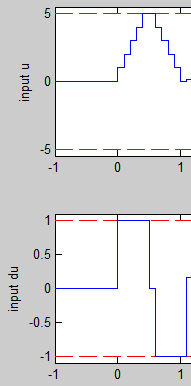
\includegraphics[width=0.5\linewidth]{10_steps.png}
\caption{Zapnuté obmedzenie}
\label{10_steps}
\end{subfigure}%
\begin{subfigure}{.5\textwidth}
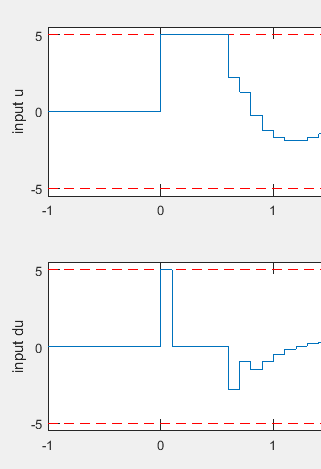
\includegraphics[width=0.7\linewidth]{11_nosteps.png}
\caption{Vypnuté obmedzenie.}
\label{11_nosteps}
\end{subfigure}
\caption{Ukážka vplyvu obmedzenia zmeny riadiaceho zásahu na časový priebeh riadiaceho zásahu.}
\end{figure}

Na základe týchto experimentov sa potvrdzujú výhody MPC regulátora, ktoré boli spomenuté v úvode ohľadne jednoduchosti zavedenia obmedzení. V tomto sa MPC viac blíži k reálnym systémom ako iné regulátory napr. PID, kde sa obmedzenia akčného zásahu musí špeciálne riešiť.

Ďalší nástroj na overenie MPC algoritmu je voľne stiahnuteľný
a~použiteľný v~prostredí Matlab. Názov je MPT toolbox. Je to dielo
inštitútu pre automatizáciu vo Švajčiarsku. Tento program je jeden
z~najpouživanejších v~prostredí Matlab.

\subsubsection{Popis systému riadenia plynovej turbíny}
Turbína s~výkonom 1,5MW obsahuje tri hlavné časti, menovite, kompresor,
spaľovaciu komorou a~vysokotlakovú turbínu. V~rokoch 1950 bolo
priemyselné využitie turbín významne rozšírené, kvôli jej nespočetným
výhodám. Napríklad neprítomnosť častí, ktoré by sa o~seba odierali,
nízka spotreba palív a~vysoká operačná spoľahlivosť. Prvá časť turbíny
zahŕňa stláčanie vzduchu na poskytnutie vysokého pomeru tlaku medzi
turbínou a~kompresorom, takže sa vzduch rozpína do turbíny. Zvyšovanie
teploty vzduchu spaľovaním paliva spôsobuje väčšie rozpínanie horúceho
vzduchu v~turbíne, poskytujúc tak potrebný výstupný výkon. Pre rôzne
prietoky vzduchu je limitovaný pomer vzduchu, ktorý môže byť dodaný, čo
je označované ako pomer palivo/vzduch. Tento faktor obmedzuje výstupný
výkon, ktorý môže byť dosiahnutý.~Maximálny pomer palivo/vzduch je
určený pracovnou teplotou lopatiek turbíny, ktoré sú vysoko stláčané.
Zaznamenanie možnej poruchy lopatiek je dôležitý problém pri monitoringu
a~detekcii chýb. Primárna požiadavka na riadenie je výstupný výkon, ale
neexistuje žiadny vhodný spôsob merania výkonu. Premenné súvisiace
s~výkonom sú riadené prostredníctvom riadenia generátora rýchlosti
N\textsubscript{g}, moduláciou prívodu paliva, kde N\textsubscript{g} je
funkciou výkonu generátora. Riadiaci zásah určuje množstvo paliva
dodávaného do motora, čo je funkciou uhla otvorenia klapky
\(\theta_{v}\left( \right).\) Parametre systému a~regulátora: rýchlosť
motora leží medzi 0 a~30~000 rpm (=500rps) táto premenná môže byť
považovaná za známu a~reprezentuje od 0 po 1.5MW. Vstup do systému je
náklon plynovej klapky 0-60°, čo je ekvivalent toku paliva 0-625kg/h.
Riadiaci rozsah výkonu je od 0 po plný výkon. Od 17~001-27~000 rpm
(283,35-450rps) je považovaný za stabilný stav rýchlosti generátora.\cite{MPC07}
\subsubsection{Identifikácia a riadenie systému plynovej turbíny}
Vstupné dáta na identifikáciu systému sú zobrazené na obrázku  \ref{12_data}. 

\begin{figure}[h]
\centering
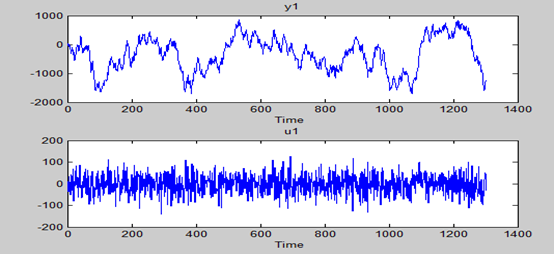
\includegraphics[width=0.9\textwidth]{12_data.png}
\caption{Časový priebeh nameraných údajov výstup a vstup systému.}
\label{12_data}
\end{figure}
Premenná y\textsubscript{1} reprezentuje výstup - otáčky motora a~u\textsubscript{1}
vstup systému - natočenie klapky. Na identifikáciu systému bol použitý Matlab nástroj \textit{ident}. Pri zisťovaní matematického modelu bolo vyskúšaných viacero metód. Najlepšie
výsledky - percento zhody nameraných a simulovaných dát dal arx model. Porovnanie nameraných a~simulovaných dát sú na
obrázku \ref{13_ident}.


\begin{figure}[h]
\centering
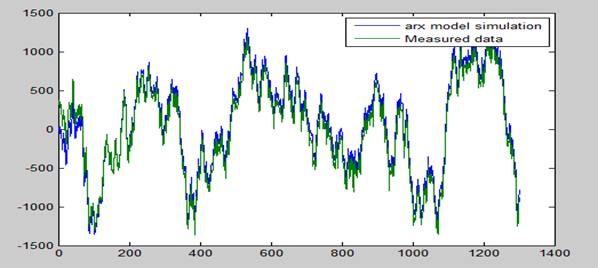
\includegraphics[width=0.9\textwidth]{13_ident.png}
\caption{Porovnanie simulovaných a nameraných údajov}
\label{13_ident}
\end{figure}
Os x predstavuje čas v sekundách a y predstavuje výstup systému. Pomocou modelu arx sa získala nasledovná prenosová funkcia

\begin{equation} \label{eq38}
\begin{split}
Gp(z) = \ \frac{Y(z)}{U(z)}
\end{split}
\end{equation}

kde
\begin{equation} \label{eq39}
\begin{split}
\text{\ Y}\left( z \right) = 2.085z^{- 1} + 0.3692z^{- 2} \\
U\left( z \right) = 1 - 0.99{13z}^{- 1} + 1.287 \times 10^{- 3}z^{- 2}
\end{split}
\end{equation}
Perióda vzorkovania je \(T_{s} = 0.25\).

Navrhnutý algoritmus bol otestovaný na reálnom systéme s~prenosovou
funkciou \ref{eq39}. Parametre simulácie sú zobrazene na obrázku \ref{15_paramt}. Časové odozvy systému s~MPC regulátorom sú
na obrázku \ref{14_simt}. Konkrétne časová odozva výstupu, v~tomto prípade
výkon motora, meraný v~rps (otáčky za sekundu) je zobrazený vo vrchnom
grafe. Vstup systému, uhol náklonu plynovej klapky meraný v~stupňoch je
v~strednom grafe a~zmena vstupu v~spodnom grafe. Všetky spomenuté
veličiny majú v~grafe modrú farbu. Zelená farba vo vrchnom grafe
predstavuje referenčný signál a~červené čiarkované čiary sú obmedzenia.

\begin{figure}[h]
\centering
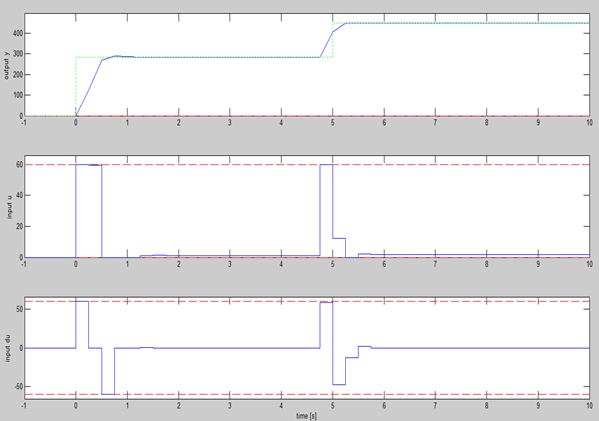
\includegraphics[width=0.9\textwidth]{14_simt.png}
\caption{Časové odozvy rýchlosti motora (v jednotkách rps) s MPC regulátorom}
\label{14_simt}
\end{figure}

\begin{figure}[h]
\centering
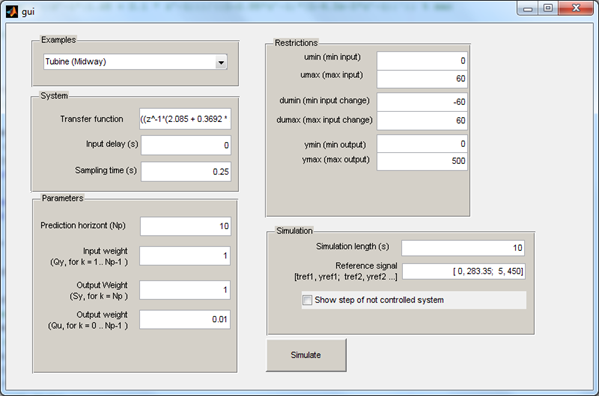
\includegraphics[width=0.9\textwidth]{15_paramt.png}
\caption{Parametre simulácie}
\label{15_paramt}
\end{figure}

renosová funkcia \ref{eq39} sa zadala do grafického rozhrania do pola
„transfer function``. Horizont predikcie bol nastavený na 10 vzoriek
dopredu. Zo simulácii vyplýva, že je to dostatočné a~efektívne, berúc do
úvahy odozvu systému a~kvalitu riadenia. Váhy boli nastavené na
prednastavené hodnoty. Obmedzenia algoritmu sú

\begin{itemize}
\item
  Na vstup 0-60 stupňov.
\item
  Zmena vstupu -60 -- 60 stupňov.
\item
  Výstup systému 0 -- 500 rps (30~000 rpm)
\end{itemize}

Referenčný signál je nastavený na hodnotu 283.35 rps v~čase 0. Po 5
sekundách je nastavený na hodnotu 450 rps.

Z~výsledkov je možné vidieť výhody prediktívneho riadenia. Keďže
prediktívny regulátor je založený na optimalizácii, je možné vidieť
minimálne akčné zásahy, čo môže viesť k~úspore spotreby.\cite{MPC08}
